

\section{Virtual reality components}



Two main subsystems, hardware and software, make up a \acrshort{vr} system. The hardware can also be divided into \acrshort{vr} engine and I/O devices, while the software can be split into application software and database as shown in Figure \ref{fig:sys}. A \acrshort{vr} system's classic five components are Software and Database, VR Engine, I/O Devices, User and Task \citep{burdea2017virtual,Bamodu2013VirtualComponents}.

\begin{figure}[ht]
    \centering
    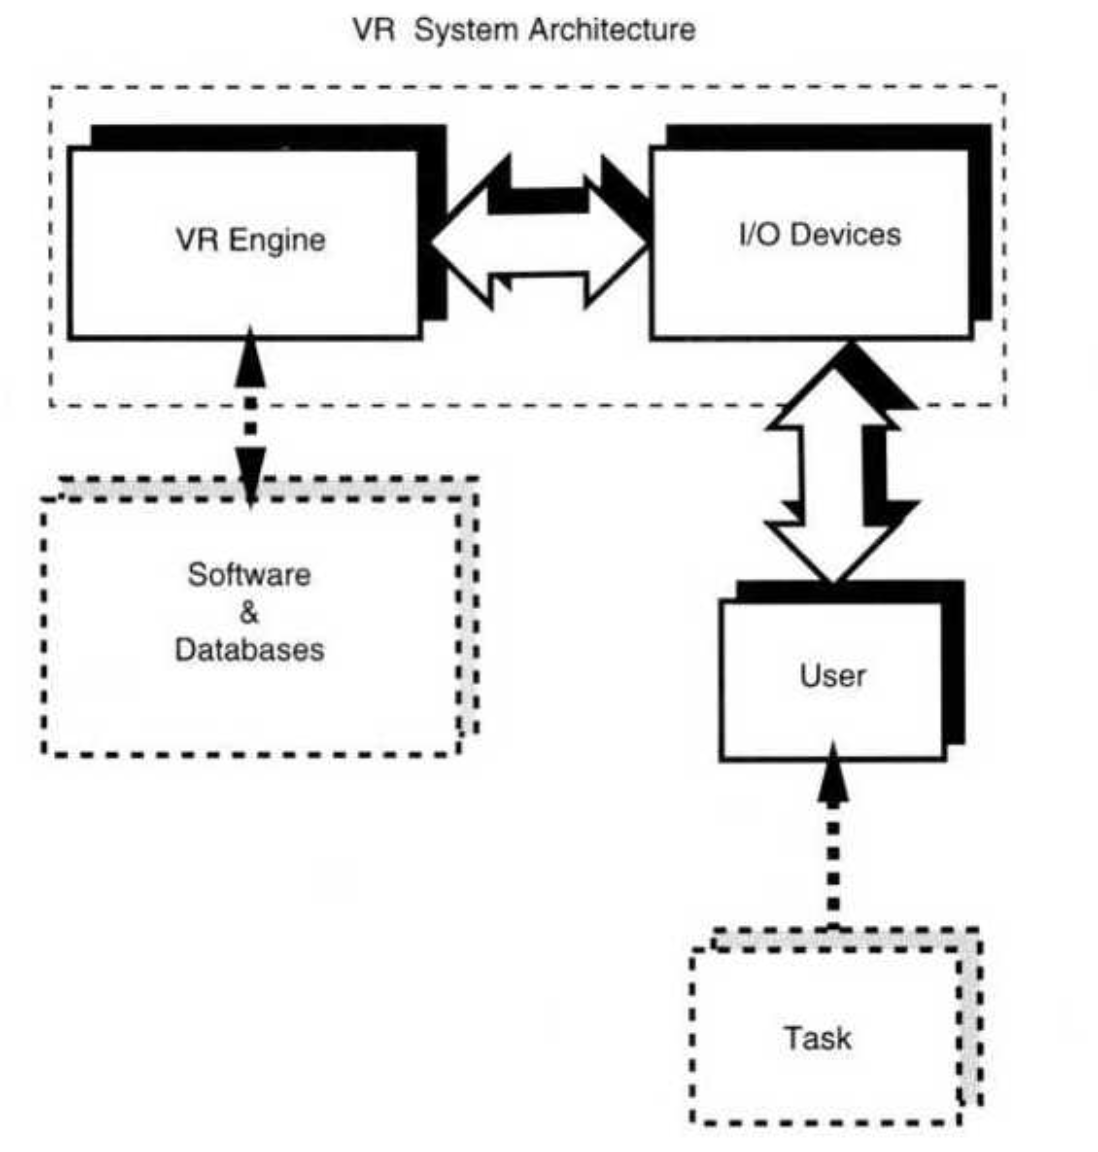
\includegraphics[width=0.50\textwidth]{images/VR.png}
    \caption{VR System Architecture - \citep{burdea2017virtual}}
    \label{fig:sys}
\end{figure}


\subsection{Software and Database}
Application for Virtual Reality Project is a set of tools and software to plan, develop and maintain virtual environments and the database where the information is stored. The tools can be classified as tools for modeling and development. There are many modeling tools available for \acrshort{vr} development, with 3D Max, Maya, and Creator being the most popular. Solidworks, Fusion 360, and CATIA are Engineering specific applications that could be used as well. \acrshort{vr} is a dynamic and integrative technology that borrows from many other innovations, such as real-time 3D computer graphics, tracking technology, motion synthesis, and haptic engineering, among others \citep{burdea2017virtual, Bamodu2013VirtualComponents}.

\subsection{VR Engine}
 The \acrshort{vr} engine or computer system must be selected in \acrshort{vr} systems according to the application's requirement. Some of the most important factors and time-consuming activity in a \acrshort{vr} environment is graphic interface and image creation. The selection of the \acrshort{vr} engine depends on the application area, user I/O devices immersion level, and the appropriate graphical output, as it is responsible for measuring and creating visual models, rendering objects, lighting, visualization, shading, simulation and show in real-time. The computer also manages interaction with users and serves as an interface to I/O devices. The processing power of the computer is a big factor to consider when choosing the \acrshort{vr} engine, and the processing power of the computer is the number of senses (graphic, audio, etc.) that can be rendered as pointed in a specific time frame. The \acrshort{vr} engine is expected to recalculate the virtual world roughly every 33ms and generate more than 24fps of real-time simulation, and the corresponding graphic engine should also be able to produce stereoscopic vision. The \acrshort{vr} engine could be a regular PC with more processing power and an efficient processor for graphics or decentralized computer systems linked through a high-speed communication network \citep{burdea2017virtual, Bamodu2013VirtualComponents}.


\subsection{I/O Devices}
 The input tools are the way for communicating with the virtual world by the user. They send signals about the user's action to the system to provide the user with appropriate reactions in real-time via the output devices. They can be categorized into devices for tracking, point-input devices, bio-controllers and voice devices. Often referred to as location sensors, tracking devices are used to detect the user's position, including electromagnetic, ultrasonic, optical, mechanical and gyroscopic detectors, data goggles, neural and bio or muscle controls. Types of point-input devices provide 6 \acrfull{dof} and space or force ball. Their technology is a normal mouse adaptation with extended functionality and 3D capability. Communication of voice is a common way of human interaction. Therefore, incorporating it into a \acrshort{vr} device also feels natural. To accomplish this, voice recognition or processing software may be used \citep{burdea2017virtual, Bamodu2013VirtualComponents} .

 The output devices receive feedback from the \acrshort{vr} engine and pass it on to users to stimulate the senses through the appropriate output devices. The possible senses-based classifications of output devices are graphics (visual), audio (aural), haptic (contact or force), odor and taste. The first 3 of these are often used in \acrshort{vr} environments, though odor and taste are still rare.The stereo video screen and the \acrfull{hmd}, which offers a higher level of immersion, are two potential traditional graphics choices. In the \acrshort{hmd}, the brain interprets the two separate views generated to provide a 3D perspective of the virtual world. An important medium in \acrshort{vr} is audio or sound, its value is only matched by that of video. To make the VR experience more immersive, 3D audio can be used to produce different sounds from different locations \citep{burdea2017virtual, Bamodu2013VirtualComponents}.



\subsection{User}

The users are the main reason to keep or to improve a particular \acrshort{vr} system design depending on their responses. Some users might have motion sickness during the simulation, therefore we should know what caused it, and how to avoid it. Human behaviour can not be measured mathematically, it is a qualitative data, therefore its more difficult to analyze the human machine interaction. \acrshort{vr} has many parameters, however \acrshort{vr} human factor studies is a series of experiments aimed at deteremined users to perform with \acrshort{vr} technology, and it tests usability, user saftey, and any related social impact related to \acrshort{vr}. 

\begin{figure}[ht]
    \centering
    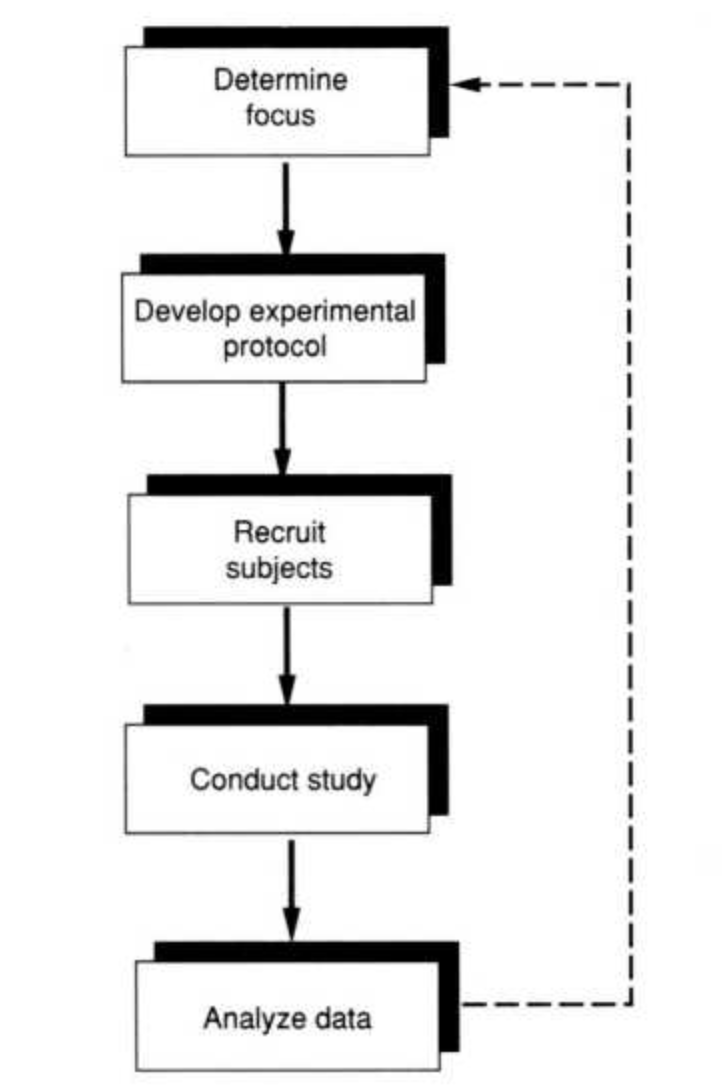
\includegraphics[width=0.40\textwidth, height=250pt]{images/VRhf.png}
    \caption{VR human factors study - \citep{burdea2017virtual}}
    \label{fig:vrhf}
\end{figure}

A great advantage of data collection in \acrlong{vr} that it can be sampled during the testing, also the researcher can have a comprehensive view while the user is immersed in the simulation. Nevertheless, while designing the experimental protocol the researcher should avoid any drawbacks, for instance to not have a repeated subject, because it will end up with the same results because data validity comes with the subject actions. Also to avoid hardware and software problems like latency which will affect the validity and reliability of the experiment. After the data is collected and analyzed, the findings will be used to refine the user interface design, enhance the software performance or add any new features to the application \citep{burdea2017virtual}. 
 
\subsection{Task}

I talked about different applications and platforms that \acrshort{vr} made an impact in it in Chapter \ref{StateoftheArt}.  


\section{Hardware and Development Environments}

In this section, I will mention and define the equipment and tools that I used to develop the application. The software that i used to build the application. and The camera's that was used to film the cities and locations in Palestine. I used Virtual reality headsets and headphones to test the application with users.


\subsection{Headsets}

\textbf{Google Cardboard}: The virtual reality platform was released in
2014 by Google. The platform is intended as a low-cost system to
encourage interest and development in VR applications. It was
named for its fold-out cardboard viewer. The Google Cardboard
headsets are built out of simple, low-cost components -
cardboard. Google open-sourced the schematics and the
assembly instructions freely on their site, allowing people to
assemble Cardboard themselves from readily available parts \citep{Prasuethsut2014GoogleReview}. The cardboards were the best option to be used for the project due to the easy mobility and the low price. It is easier to travel with it through airports or checkpoints since it’s cardboard.




\textbf{Google Daydream}: The virtual reality platform was released in
2014 by Google. The platform is intended as a low-cost system to
encourage interest and development in VR applications. It was
named for its fold-out cardboard viewer. The Google Cardboard
headsets are built out of simple, low-cost components -
cardboard. Google open-sourced the schematics and the
assembly instructions freely on their site, allowing people to
assemble Cardboard themselves from readily available parts \citep{Prasuethsut2014GoogleReview}. The
cardboards were the best option to be used for the project due to the easy mobility and the
low price. It is easier to travel with it through airports or checkpoints since it’s cardboard.



\subsection{Cameras}
\textbf{GoPro Fusion}: the footage quality can reach up to 5.2K spherical video
resolution. The GoPro fusion can be controlled via a mobile
application through Bluetooth or Wi-Fi. The two lenses on the two
sides are not symmetrically aligned, they are off-axis. That helps to
process the images or the footage taken from the two lenses to not
have visible stitching or overlapping in the final image. That is a
common problem in most of the VR cameras to have a big overlapping on the final image. The
data is saved on two microSD cards one for each lens, the files need to be combined to have
a final 360$^{\circ}$ video \citep{Easton2018}. The camera was used in most of the project filming material,
it has the best footage quality and a perfect stabilization in the videos.


\textbf{Samsung Gear 360}: The small and rounded shape of the camera is ideal for
handheld shooting, although it has a socket also for a tripod. A small LCD
screen helps in navigating through the camera modes. The video resolution is
4K, while the still images are somewhat soft. The smartphone app is easy to
use and clear for the user also it offers a good range of viewing options. In
general is it a small and simple camera to use \citep{DigitalCamera2018}. The
camera used as a backup camera during the project. The quality is acceptable
for a small and very light camera.

\subsection{Development Environments}

The VR technology is moving forward and there is an increasing number of tools and platforms
available for developers (“11 Tools for VR Developers,” 2017). VR technology has found its
way into different environments like computers, smartphone, and web. This section will
mention the two tools that were used by the VR team developers to build a mobile VR
application and a VR experience over the web. Nevertheless, most browsers are still struggling
with the headset device support. Most phones can be detected with the WebVR-polyfill and
if turned sideways, it will switch the dual display mode automatically that you can use Google
Cardboard or other headsets built for smartphones (“11 Tools for VR Developers,” 2017).


\textbf{Unity 3D}: Unity is one of the most famous game engines, it has a direct VR mode to preview
the work on any Head mounted display, which can be easier and faster for designers to boost
their productivity. Most of the Head mounted displays are supported in Unity. Unity works
with C\# and JavaScript; it is easy to learn due to the huge online community. Unity can export
the work to almost any platform even WebGL (“11 Tools for VR Developers,” 2017). Unity was
the best and most powerful tool to be used during the project to develop the VR experience.
Due to the easy implementation of the VR Environment in Unity, also the variety of platforms
that it allows the developer to distribute the software on it. In addition, there is a huge
community for Unity developers on the internet, where everyone can share knowledge and
expertise.

\section{Development \& Implementation}

 Also, I will present how I did manage to re-build part of the Al-Ghabisiyya village. These tools helped me in modeling the terrain of the geographical area as well as re-building most of the houses of Al-Ghabisiyya. Placing the village on the right location of the map was tricky and challenging therefore, I will explain it in detail. 

\subsection{Glimpses from Palestine Application}





\subsection{User Interface}

“ In order to allow human-computer interaction it is necessary to use special interfaces designed to input a user's commands into the computer and to provide feedback from the simulation to the user” \citep{burdea2017virtual}.